\documentclass[11pt]{article}
\usepackage{fullpage}
\usepackage{amsthm}
\usepackage{amsmath} \usepackage{amssymb}
\usepackage{graphicx}

\graphicspath{ {./imgs/} }

\setlength{\parindent}{0pt}

\title{Introduction to Machine Learning (CO395)}
\author{Michael Tsang}

\newtheorem{defn}{Definition}
\newtheorem{eg}{Example}
\newtheorem{theo}{Theorem}
\newtheorem{lem}{Lemma}

\begin{document}

\maketitle
\section{Machine Learning}
\textit{The field of machine learning is concerned with the question of how to construct computer programs that automatically improve with experience.}

\subsection{Supervised Learning}
\begin{defn}
Learning an unknown mapping $f(x_i) = y_i$ from training data, given in the form of input  and output pairs $D = \{ (x_i, y_i) \}^N_{i = 1}$.
\end{defn}

\begin{itemize}
  \item $D$ is the \textbf{training set}, $N$ is the number of training examples/samples/data points. 
  \item The $x_i$ are in the \textbf{feature space} $\mathcal{X}$ and the $y_i \in \mathcal{Y}$ are in the \textbf{label space}.
  \item In the simplest setting, each training input $x_i$ is a $D$-dimensional vector of numbers, these are called \textbf{features}, \textbf{attributes}, or \textbf{covariates}.
  \item In general, $x_i$ could be a complex structured object, such as an image or sentence.
\end{itemize}

\subsubsection{Spaces}
\begin{figure}[h]
  \caption{Spaces before the \textit{Deep Learning Era}.}
  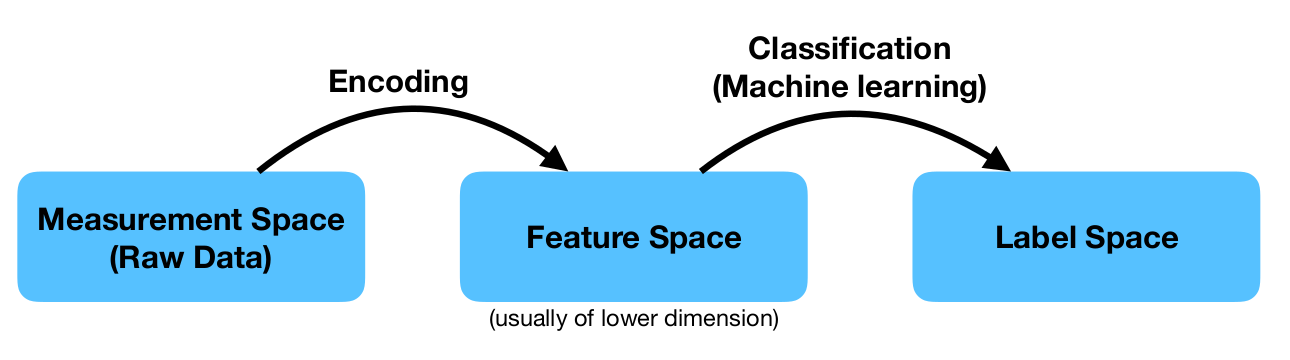
\includegraphics[scale=0.2]{spacesbefore}
  \centering
\end{figure}

\begin{figure}[h]
  \caption{Spaces after the \textit{Deep Learning Era}.}
  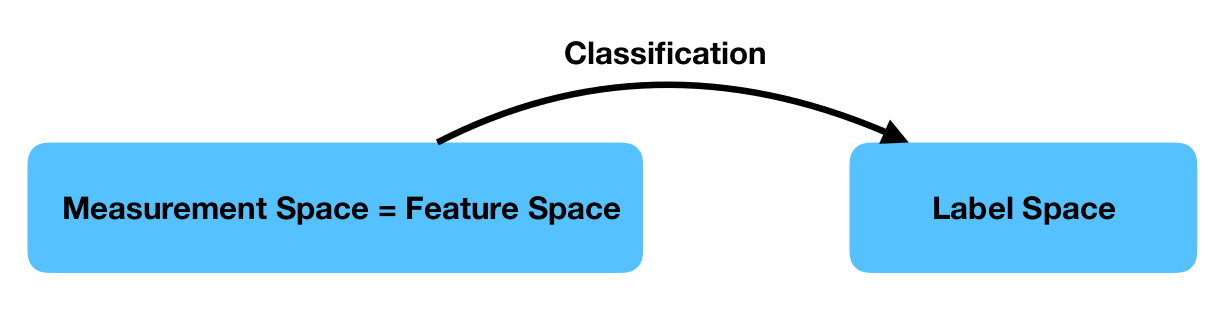
\includegraphics[scale=0.2]{spacesafter}
  \centering
\end{figure}

\subsubsection{Label Space}
There are three main types of \textbf{Label Spaces}:
\begin{itemize}
  \item \textbf{Categorical} (also called class) - $y_i$ is a categorical or nominal variable from some finite set $y_i \in \{1, \ldots, C \}$ (e.g.\ ``Apple'', ``Banana''.).
    The supervised learning task is known as \textbf{classification} or \textbf{pattern recognition}.
  \item \textbf{Real-valued Scalar} - e.g.\ credit score, the task is known as \textbf{regression} or \textbf{function approximation}.
  \item \textbf{Ordinal Regression} - this occurs when the label space has some natural ordering which can be approximated as a regression problem that is subsequently discretised, e.g.\ school grades.
\end{itemize}

\subsection{Unsupervised Learning}
\begin{defn}
Discovering an underlying, hidden, or latent structure within the data $x$.
\end{defn}

The aim is to find a structure that explains the data in a more efficient way.
We can think of this as reducing the amount of bits to store the important features of the data, akin to lossy data compression. \\

This is possible in broadly two ways:
\begin{itemize}
  \item \textbf{Dimensionality reduction} - reducing the dimensions in the data.
  \item \textbf{Clustering} - assigning the data to automatically defined categorical labels.
\end{itemize}

\subsection{Reinforcement Learning}
\begin{defn}
Finding which action to take in order to maximise the received rewards.
\end{defn}

The main differences are:
\begin{itemize}
  \item The best or correct solution is not given to the agent, only a reward signal.
  \item Feedback is delayed.
  \item Time matters, data is sequential.
  \item Agent's decisions affect the subsequent received data.
\end{itemize}

An example of this is in a moving robot.

\subsection{Main Problems in Machine Learning}
\begin{itemize}
  \item \textbf{Classification} - predicting the right label for an unknown sample.
  \item \textbf{Regression} - approximating an unknown function.
  \item \textbf{Clustering} - grouping data in such a way that data points in the same group (cluster) are more similar to each other than to those in other clusters.
  \item \textbf{Dimensionality Reduction} - reducing the dimensionality of the observed data.
  \item \textbf{Density Estimation} - estimating an unobservable underlying probability density function based on observed data.
  \item \textbf{Policy Search} - finding which action an agent should take, depending on its current state, to maximise the received rewards.
\end{itemize}

\section{Instance Based Learning}
We need large amounts of data to make accurate predictions; selecting the right features and representation is crucial.

\subsection{$k$-Nearest Neighbours}
One way of implementing a classifier is to consider the $k$-nearest neighbours in the feature space of the current instance, and \textbf{assign the class in the majority}.

We define the nearest neighbours of a query instance $x_q$ in terms of the Euclidean distance ($L2$-norm):
\[
  d(x_i, x_q) = \sqrt{\sum_g (a_g(x_i) - a_g(x_q))^2}
\]
where the instances $x_i$ belong to the dataset, and all instances are described with a set of $g = [1, \ldots, p]$ features $a_g$.

Alternatively we could use different definitions of distance:
\begin{itemize}
  \item Manhattan ($L1$-norm)
    \[
      d(x_i, x_q) = \sum_g \lvert a_g(x_i) - a_g(x_q) \rvert
    \]
  \item Chebyshev ($L^\infty$-norm)
    \[
      d(x_i, x_q) = \max \lvert a_g(x_i) - a_g(x_q) \rvert
    \]
\end{itemize}

\subsubsection{Choice of $k$}
\begin{itemize}
  \item Small $k$ - Good resolution of class borderlines, but sensitive to noise.
  \item Large $k$ - Bad resolution of class borderlines, but robust to noise.
\end{itemize}

We choose a value of $k$ with a validation dataset.

While the $k$-NN algorithm is powerful, finding the nearest neighbours can be slow if the dataset is large.
Approaches to improve this include: $k$-d trees; Locality-Sensitive hashing with hash tables; or generating prototypes with Learning Vector Quantisation.

\subsection{Distance-Weighted $k$-NN Algorithm}
We assign a weight $w_r$ to each neighbour $x_r$ of the query instance $x_q$ based on the distance $d(x_r, x_q)$: \textbf{nearer neighbours have greater weight}.

Any measure favouring the votes of nearby neighbours works:
\begin{itemize}
  \item Inverse of the distance
    \[
      w_r = \frac{1}{d(x_r, x_q)}
    \]
  \item Gaussian distribution
    \[
      w_r = \frac{1}{\sqrt{2 \pi}} \exp \left(\frac{-d(x_r, x_q)^2}{2}\right)
    \]
\end{itemize}

The value of $k$ is less important as distance examples will have small weight and not greatly affect the classification.

If $k = n$, where $n$ is the total number of instances, the algorithm is a \textbf{global method}.
Otherwise if $k < n$, it is a \textbf{local method}, only takes into account some of the instances. \\

Since classification is based on a weighted combination of all $k$-NN, then the impact of noise is smoothed out - the distance-weighted $k$-NN is \textbf{robust to noisy training data}.

Since the distance is based on all features of each instance, irrelevant features may cause instances that belong in the \textbf{same class to be distant from one another}. \\

To remedy this, we \textbf{weight each feature} differently when calculating the distance.

\subsection{Curse of Dimensionality}
\begin{figure}[h]
  \caption{The relationship between average distance and dimensions.}
  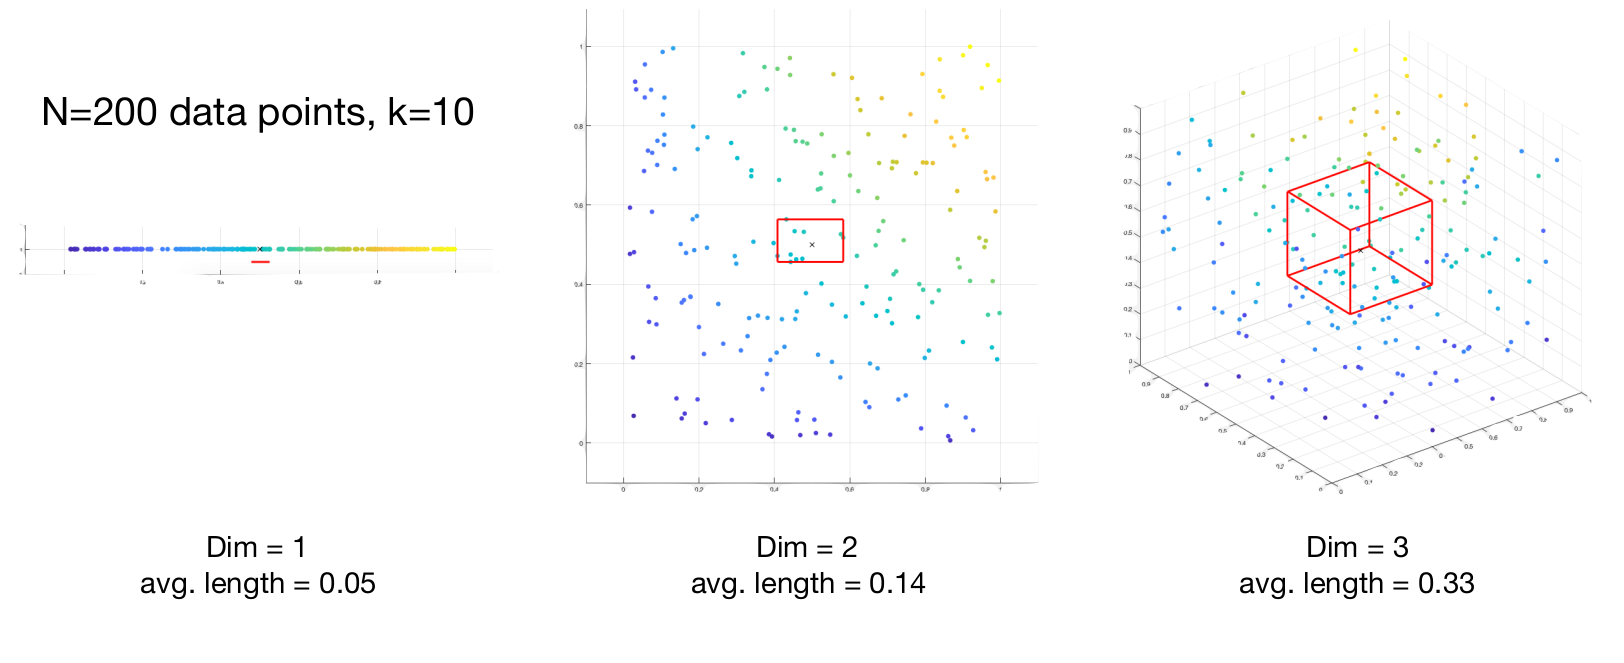
\includegraphics[scale=0.3]{curseofdim}
  \centering
\end{figure}

As the dimensions of the feature space increases, the distance to the nearest neighbours increases.

\subsection{$k$-NN for Regression}
Instead of using the class in the majority, we consider the \textbf{value} in the majority.

In distance-weighted $k$-NN, the prediction of the algorithm is the \textbf{weighted average value} of the $k$-NN.

This is also known as \textit{Locally Weighted Regression}.

\subsection{Lazy Learning}
\begin{defn}
Data is stored, but generalising beyond this is postponed until an explicit request is made.
\end{defn}

\begin{enumerate}
  \item Search the memory for similar instances.
  \item Retrieve the related solutions.
  \item Adapt solutions to the current instance.
  \item Assign estimated solution to the current instance.
\end{enumerate}

An example of this is the $k$-NN algorithm.

\begin{itemize}
  \item A \textbf{different approximation to the target function} is constructed for each query instance.
  \item The collection of \textbf{less complex local approximations} represents a complex target function, where the problem domain could be incomplete.
  \item Large space requirement to store the entire training dataset, with long query time.
  \item Most useful for large datasets with few attributes.
\end{itemize}

\subsection{Eager Learning}
\begin{defn}
  A general, explicit description of the target function is constructed, based on the provided training examples.
\end{defn}

Examples of this are in artifical neural networks and decision trees.

\begin{itemize}
  \item The \textbf{same approximation to the target function} is used, which must be learned based on training examples, and before input queries are observed.
  \item Better memory efficiency, and usually low query time.
  \item Deals better with noise.
  \item Generally unable to provide good local approximations in the target function.
\end{itemize}


\end{document}
